\documentclass[letterpaper]{article}
\usepackage[margin=1in]{geometry}
\usepackage[utf8]{inputenc}
\usepackage{textcomp}
\usepackage{amssymb}
\usepackage{natbib}
\usepackage{graphicx}
\usepackage{gensymb}
\usepackage{amsthm, amsmath, mathtools}
\usepackage[dvipsnames]{xcolor}
\usepackage{enumerate}
\usepackage{mdframed}
\usepackage[most]{tcolorbox}
\usepackage{csquotes}
% https://tex.stackexchange.com/questions/13506/how-to-continue-the-framed-text-box-on-multiple-pages

\tcbuselibrary{theorems}

\newcommand{\R}{\mathbb{R}}
\newcommand{\Z}{\mathbb{Z}}
\newcommand{\N}{\mathbb{N}}
\newcommand{\Q}{\mathbb{Q}}
\newcommand{\C}{\mathbb{C}}
\newcommand{\code}[1]{\texttt{#1}}
\newcommand{\mdiamond}{$\diamondsuit$}
\newcommand{\PowerSet}{\mathcal{P}}
\newcommand{\Mod}[1]{\ (\mathrm{mod}\ #1)}
\DeclareMathOperator{\lcm}{lcm}

%\newtheorem*{theorem}{Theorem}
%\newtheorem*{definition}{Definition}
%\newtheorem*{corollary}{Corollary}
%\newtheorem*{lemma}{Lemma}
\newtheorem*{proposition}{Proposition}


\newtcbtheorem[number within=section]{theorem}{Theorem}
{colback=green!5,colframe=green!35!black,fonttitle=\bfseries}{th}

\newtcbtheorem[number within=section]{definition}{Definition}
{colback=blue!5,colframe=blue!35!black,fonttitle=\bfseries}{def}

\newtcbtheorem[number within=section]{corollary}{Corollary}
{colback=yellow!5,colframe=yellow!35!black,fonttitle=\bfseries}{cor}

\newtcbtheorem[number within=section]{lemma}{Lemma}
{colback=red!5,colframe=red!35!black,fonttitle=\bfseries}{lem}

\newtcbtheorem[number within=section]{example}{Example}
{colback=white!5,colframe=white!35!black,fonttitle=\bfseries}{def}

\newtcbtheorem[number within=section]{note}{Important Note}{
        enhanced,
        sharp corners,
        attach boxed title to top left={
            xshift=-1mm,
            yshift=-5mm,
            yshifttext=-1mm
        },
        top=1.5em,
        colback=white,
        colframe=black,
        fonttitle=\bfseries,
        boxed title style={
            sharp corners,
            size=small,
            colback=red!75!black,
            colframe=red!75!black,
        } 
    }{impnote}
\usepackage[utf8]{inputenc}
\usepackage[english]{babel}
\usepackage{fancyhdr}
\usepackage[hidelinks]{hyperref}

\pagestyle{fancy}
\fancyhf{}
\rhead{Math 170B}
\chead{Friday, April 21, 2023}
\lhead{Lecture 9}
\rfoot{\thepage}

\setlength{\parindent}{0pt}

\begin{document}

\section{Fixed Point and Functional Iteration (Section 3.4)}
Let $F$ be a one-dimensional real-valued (and typically continuous) function. Then, the \textbf{functional iteration} is defined by 
\[x_{m + 1} = F(x_m), \quad m \geq 0.\]
Note that this generalizes the previous approaches that we've had; for example, we can represent Newton's method in this way. 

\begin{mdframed}
    (Example.) Consider Newton's method. We can write 
    \[x_{m + 1} = \underbrace{x_{m} - \frac{f(x_m)}{f'(x_m)}}_{F(x_m)}.\]
\end{mdframed}
If the limit, $\lim_{n \mapsto \infty} x_{m + 1} = s$ exists, then 
\[s = \lim_{m \mapsto \infty} x_{m + 1} = \lim_{m \mapsto \infty} F(x_m) = F\left(\lim_{m \mapsto \infty} x_m\right) = F(s).\]
The fixed point, $s$, is defined by $\boxed{s = F(s)}.$

\subsection{Contractive Mapping Property}
Let $F$ be a map on a closed set $C \subseteq \R$ into itself. For $0 < \lambda < 1$, we have \[\boxed{|F(x) - F(y)| \leq \lambda |x - y|}\] for $x, y \in C$. In other words, a mapping (or function) $F$ is said to be \textbf{contractive} if there exists a $\lambda$ such that the above is satisfied.
\begin{center}
    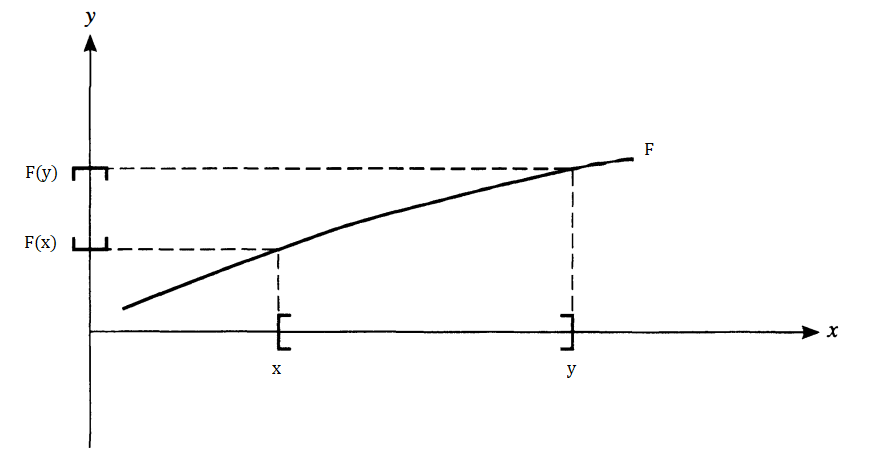
\includegraphics[scale=0.8]{../assets/contractive.png}
\end{center}
The interval between $x$ and $y$ is larger than the interval between $F(x)$ and $F(y)$ because $\lambda \leq 1$ (i.e., the intervals are being shrunk).

\begin{theorem}{Contractive Mapping Theorem}{}
    Let 
    \begin{itemize}
        \item $C$ be a closed subset of $\R$ (i.e., $C \subseteq \R$),
        \item $F$ be a contractive mapping from $C$ into $C$, and 
        \item $x_0 \in C$ be a starting point. 
    \end{itemize}
    Then, $x_{m + 1} = F(x_m)$ converges to a unique fixed point $s$ starting from $x_0$.
\end{theorem}
\begin{proof}
    We'll prove both the convergence and uniqueness parts of the theorem.
    \begin{description}
        \item[Convergence:] We have 
        \[\begin{aligned}
            |x_{m + 1} - x_m| = |F(x_m) - F(x_{m - 1})| &\leq \lambda |x_m - x_{m - 1}| \\ 
                &\leq \lambda^2 |x_{m - 1} - x_{m - 2}| \\ 
                &\vdots \\ 
                &\leq \lambda^m |x_1 - x_0|.
        \end{aligned}\]
        Then, \[\sum_{m = 0}^{\infty} |x_{m + 1} - x_m| \leq \sum_{m = 0}^{\infty} \lambda^m |x_1 - x_0| = \frac{|x_1 - x_0|}{1 - \lambda}.\]
        Thus, \[\lim_{m \mapsto \infty} x_{m + 1} = \lim_{m \mapsto \infty} x_m = s\] converges. This proves the convergence part. 

        \item[Uniqueness:] Suppose we have two fixed points $s_1$ and $s_2$, and $0 < \lambda < 1$. Then, \[|F(s_1) - F(s_2)| \leq \lambda |s_1 - s_2|.\]
        But, if $s_1$ and $s_2$ are two fixed points, then we have $F(s_1) = s_1$ and $F(s_2) = s_2$. So, 
        \[|s_1 - s-2| \leq \lambda |s_1 - s_2|.\]
        Note that this can only hold if $s_1 = s_2$, as $\lambda = 1$ but remember that $\lambda < 1$. 
    \end{description}
    Then, we're done. 
\end{proof}

\begin{mdframed}
    (Example.) Suppose we want to prove convergence for $x_{m + 1} = 3 - \frac{1}{3} |x_m|$, with $x_0 = -15$ and $m \geq 0$. 

    \bigskip 

    Let $F(x) = 3 - \frac{1}{3}|x|$. If we plot $F(x)$, we get 
    \begin{center}
        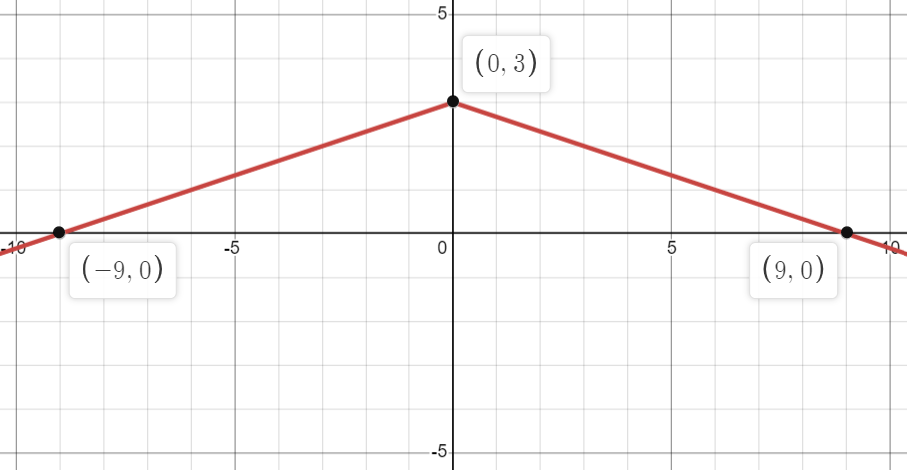
\includegraphics[scale=0.7]{../assets/contractive_ex1.png}
    \end{center}
    Notice how $F$ maps real values back to real values. Note that $C = \R$ and $x_0 \in C$. Now, we want to check the contraction property. If $x, y \in C$, then \[|F(x) - F(y)| = \left|\left(3 - \frac{1}{3}|x|\right) - \left(3 - \frac{1}{3}|y|\right)\right| = \frac{1}{3}\left||x| - |y|\right|.\]
    Applying the triangle inequality, we have 
    \[\frac{1}{3}\left||x| - |y|\right| \leq \frac{1}{3}|x - y|.\]
    So, if we set $\lambda = \frac{1}{3} < 1$, then we've shown the contractive property. 

    \bigskip 

    Now, we want to think about the fixed point case. Since $x_{m + 1}$ converges, we have a fixed point. The fixed point is defined by 
    \[s = F(s).\]
    So, $s = 3 - \frac{1}{3}|s|$. Then, solving for $s$ gives us the fixed points. Since we have absolute values, we have two cases to consider. 
    \begin{itemize}
        \item $s = 3 - \frac{1}{3}s$ if $s > 0$.
        \[\frac{4}{3}s = 3 \implies s = \frac{9}{4}.\]
        \item $s = 3 + \frac{1}{3}s$ if $s < 0$.
        \[\frac{2}{3}s = 3 \implies s = \frac{9}{2}.\]
    \end{itemize}
    Notice how we have 2 values of $s$. We have two equations above, but notice how the second equation cannot be true as the equation is only value if $s < 0$, but we have $s = \frac{9}{2} > 0$. Thus, $s = \frac{9}{4} \in C$ is our fixed point. 
\end{mdframed}

\begin{mdframed}
    (Example.) Suppose we have \[F(x) = 4 + \frac{1}{3}\sin(2x),\] and let $C = \left[\frac{11}{3}, \frac{13}{3}\right].$ To consider the contraction property for this function, we can apply the Mean-Value Theorem. Let $x, y \in C$. Then, 
    \[\begin{aligned}
        |F(x) - F(y)| &= \left|\left(4 + \frac{1}{3}\sin(2x)\right) - \left(4 + \frac{1}{3}\sin(2y)\right)\right| \\ 
            &= \frac{1}{3}|\sin(2x) - \sin(2y)| && \text{Mean-Value Theorem}
            &= \frac{1}{3}|2\cos(2\xi)(x - y)| \\ 
            &\leq \frac{2}{3}\left|x - y\right|.
    \end{aligned}\]
    From there, it's clear that $\lambda = \frac{2}{3} < 1$. 

    \bigskip 

    Note that we can write a program to compute this fixed point based on this simple algorithm. 
    \begin{algorithm}[H]
        \caption{Computing Fixed Point}
        \label{alg:two}
        \begin{algorithmic}[1]
            \State $x \gets 4$
            \State $M \gets 20$

            \For{$k \gets 1$ to $M$}
                \State $x \gets 4 + \frac{1}{3}\sin(2x)$
            \EndFor 
        \end{algorithmic}
    \end{algorithm}
    Here, $x$ will contain the approximate fixed point.
\end{mdframed}


\end{document}